\documentclass{beamer}

\usepackage{gensymb}
\usepackage{transparent}
\input{entete_beamer_pdflatex}
\usepackage{listings}
\usepackage[babel=true]{csquotes}
\lstset{language=Python, tabsize=2, breaklines=true, showstringspaces=false}

\useoutertheme{infolines}
\setbeamersize{text margin left=1cm,text margin right=1cm}

\title{Presentation de projet de SI}
\subtitle{Tropodrone}
\author{Gueydan Noé, Manceau Thibaut, Gros Alexis, Porteries Tristan}

\usebackgroundtemplate%
{%
    {\transparent{0.3}\includegraphics[width=\paperwidth,height=\paperheight]{../Images/structure1_1.PNG}}%
}

\begin{document}

\begin{frame}
  \titlepage
\end{frame}

\begin{frame}
    \frametitle{Sommaire}
    \begin{multicols}{2}
      {
		\setcounter{tocdepth}{1}
        \tableofcontents
      }
    \end{multicols}
\end{frame}

\section{Introduction}

\subsection{Idée}
\begin{frame}{Idée}
 Fusionner un drone avec un dirigeable.

 Pourquoi~?~:
 \begin{itemize}
  \item augmenter l'autonomie des drones~;
  \item réduire la dangerosité des drones~;
  \item augmenter la charge utile.
 \end{itemize}
\end{frame}

\subsection{Objectif}
\begin{frame}{Objectif du projet}
  Créer une structure composée de ballons contenant un gaz plus léger que l’air qui soutient une partie ou la totalité du poids d'un drone.
\end{frame}

\subsection{Contraintes et besoins}
\begin{frame}{Contraintes et besoins}
	\begin{itemize}
		\item garder la manoeuvrabilité du drone~;
		\item porter une charge utile~;
		\item ballons avec force d'élévation suffisante.
	\end{itemize}

\end{frame}

\subsection{Drone}

\begin{frame}{Modèle de drone choisi}
  \begin{multicols}{2}
    Drone XCSOURCE~: \\
    \begin{itemize}
      \item 290 mm diagonale~;
      \item 190 mm longueur~;
      \item 70 mm hauteur~;
      \item moteur EMAX MT2204 2300KV Brushless Motor~;
      \item Accu Lipo Gens Ace 2200Mah 11.1V 25C 3S~;
      \item 450 g.
    \end{itemize}
    \newpage
    \begin{center}
      \includegraphics[width=6cm]{../Images/drone.JPG}
    \end{center}
    \captionof{figure}{Drone XCSOURCE.}
  \end{multicols}
\end{frame}

\section{Élévation}

\subsection{Gaz}

\begin{frame}{Calcul de la capacité d'élévation}
	Gaz plus léger que l'air pour utiliser poussée d'archimède~(Pa).\\
  Calcul de la capacité d'élévation (Ce)~:
	\begin{center}
		\boxed{Pa = Masse Volumique Air \times g}
		\boxed{Ce = \frac{Pa - P}{g}}
	\end{center}

	\begin{tabular}{|l|c|c|c|}
		\hline
		Gaz & Air & Hydrogène & Hélium \\
		\hline
		Masse Volumique $(kg.m^3)$ & 1.29 & 0.08988 & 0.1785 \\
		\hline
		Force d'élévation $(N.m^3)$ & 0 & 11.77 & 10.90 \\
		\hline
	\end{tabular}

\end{frame}

\section{Ballons}

\subsection{Matériau}

\begin{frame}{Choix du matériau}
	\begin{tabular}{|l|p{0.35\linewidth}|p{0.35\linewidth}|}
		\hline
		Matériaux & Avantages & Inconvénients \\
		\hline

		Latex &
		Facile à trouver dans le commerce &
		Seulement en forme sphérique~; peu étanche \\
		\hline

		Hypalon & Étanche & Introuvable dans le commerce~; fragile aux ultraviolets \\
		\hline

		Mylar &
		Facile à trouver dans le commerce~; résistant à la traction~; peut être assemblé~; léger~: $17 g.m^{-2}$ &
		Raide~; fragile au cisaillement et à la perforation\\
		\hline
	\end{tabular}
\end{frame}

\subsection{Colles}

\begin{frame}{Collage du mylar}
	\begin{tabular}{|l|l|}
		\hline
		Colles & \\
		\hline
		401 & adhérent~; Facile à appliquer~; Peu résistant au pelage. \\
		\hline
		Néoprène & Difficile à appliquer~; Résistant au pelage. \\
		\hline
		330 & Peu adhérent. \\
		\hline
 \end{tabular}

 \begin{center}
		\includegraphics[width=5cm]{../Images/test_colle.jpg}
 \end{center}
\end{frame}

\begin{frame}{Problème du collage}
  Collage du ballon extérieur~: contrainte de pelage, pire situation.
  \begin{center}
    \includegraphics[width=5cm]{../Images/colle_pelage.png}
    \includegraphics[width=5cm]{../Images/colle_cisaillement.png}
  \end{center}
  Solution~: coller la couture sur le ballon.
\end{frame}

\begin{frame}{Tests de traction et pelage avec 401}
   \begin{center}
    \begin{tabular}{|c|c|}
      \hline
      Pelage & Cisaillement \\
      \hline
      $0.45 N.cm^{-2}$ & $12.1 N.cm^{-2}$ \\
      \hline
    \end{tabular}
  \end{center}
  \begin{center}
    \includegraphics[width=5cm]{../Images/test_cisaillement.png}
    \includegraphics[width=5cm]{../Images/test_pelage.png}
  \end{center}
\end{frame}

\subsection{Volume}

\begin{frame}{Bilan des masses et du volume}
	\begin{center}
		\begin{tabular}{|c|c|c|c|}
			\hline
			Élément & Drone & Ballon & Total \\
			\hline
			Masse (en g) & 450 & 300 & 750 \\
			\hline
		\end{tabular}

	\end{center}

  Volume d'hélium nécessaire~: $0.75 m^3$

  Volume des ballons~: $0.25 m^3$
\end{frame}


\subsection{Forme}

\begin{frame}{Choix et calcul de la forme}
	Forme composée de deux cônes et d'un parallépipède central. Angle de $60\degree$ entre les ballons.
	\begin{center}
		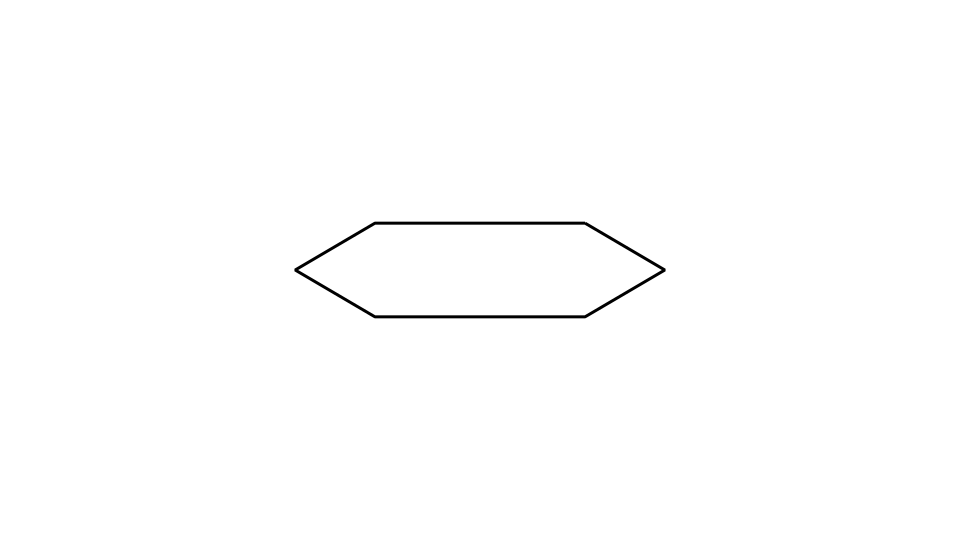
\includegraphics[width=6.5cm]{../Images/ballon.png}
		\includegraphics[width=3.5cm, angle=90]{../Images/plan_ballon.png}
	\end{center}
\end{frame}



\subsection{Assemblage}

\begin{frame}{Assemblage des ballons}
	\begin{tabular}{cc}
		\includegraphics[width=5cm]{../Images/assen_1.JPG} &
		\includegraphics[width=5cm]{../Images/assen_3.JPG} \\
		\includegraphics[width=3cm]{../Images/assen_2.JPG} & \\
	\end{tabular}

\end{frame}


\section{Structure}

\subsection{Contraintes}

\begin{frame}{}
  Contraintes de la structure~:
 \begin{itemize}
  \item 3 axes de liberté~;
  \item adaptée au drone~;
  \item légèreté.
 \end{itemize}

\end{frame}


\subsection{Ancienne structure}

\begin{frame}{Première structure}
 \begin{center}
	Drone suspendu au milieu d'un gyroscope.
  \includegraphics[width=8cm]{../Images/structure0_0.jpg}
 \end{center}
 Inconvénients~: lourd et complexe.
\end{frame}


\subsection{Nouvelle structure}

\begin{frame}{Structure finale}
 \begin{center}
	Drone suspendu entre deux tétraèdres.
  \includegraphics[width=8cm]{../Images/structure1_0.PNG}
 \end{center}
 Avantages~: léger et simple.
\end{frame}

\begin{frame}
 \begin{center}
		\includegraphics[width=10cm]{../Images/structure1_1.PNG}
 \end{center}
\end{frame}


\section{Aérodynamisme}

\subsection{Équation de traînée}
\begin{frame}{Équation de traînée}
 But : que le drone soit le moins sensible à l'air possible \\
 Force de traînée matérialisée par l'équation \\
 \begin{center}
  \boxed{\displaystyle{\frac12 \times \rho \times S \times Cx \times V^2}}
 \end{center}
 Avec~:
 \begin{itemize}
  \item $\rho$ la masse volumique du fluide dans lequel a lieu le déplacement en $kg.m^{-3}$~;
  \item S la surface~;
  \item Cx le coefficient de traînée~;
  \item V la vitesse relative du mobile par rapport au fluide en $m.s^{-1}$.
 \end{itemize}
\end{frame}

\subsection{Résolution sous SW - 1}
\begin{frame}{Résolution sous SW dans différentes conformations}
	\begin{center}
		\begin{tabular}{c}
      \includegraphics[width=10cm]{../Images/Capture.PNG} \\
			\includegraphics[width=8cm]{../Images/resultatsSimulationSW.png}
		\end{tabular}
	\end{center}
\end{frame}

\subsection{Résolution sous SW - 2}
\begin{frame}{Résolution sous SW dans différentes conformations}
 \begin{center}
	\includegraphics[width=10cm]{../Images/visualisationSimulationSW.PNG} \\
 \end{center}
\end{frame}


\end{document}
